\documentclass[10pt]{beamer}

\usetheme{metropolis}
\usepackage{appendixnumberbeamer}

\usepackage{booktabs}
\usepackage[scale=2]{ccicons}

\usepackage{pgfplots}
\usepgfplotslibrary{dateplot}

\usepackage{xspace}
\newcommand{\themename}{\textbf{\textsc{metropolis}}\xspace}

\title{Kinetic Molecular Theory and the Boltzmann Distribution}
\subtitle{Unit 3: Intermolecular Forces and Properties}
\date{\today}
\author{AP Chemistry}
% \titlegraphic{\hfill\includegraphics[height=1.5cm]{logo.pdf}}

\begin{document}

\maketitle

\begin{frame}[standout]
\textbf{\textsc{Journal:}}
 \textbf{How would you define the differences between solids, liquids, and gases? (5 minutes)} 
\end{frame}

\begin{frame}{Review: Solids, Liquids, and Gases}
  \begin{figure}
    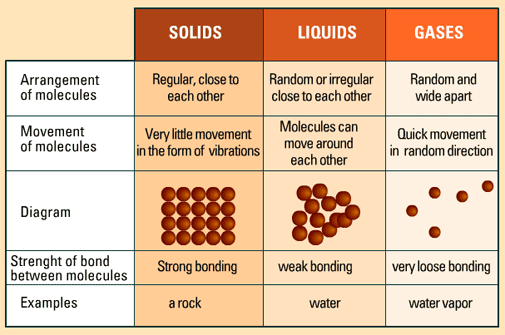
\includegraphics[scale=0.6]{3_intermolecular_forces/slg.png}
  \end{figure}
\end{frame}

\begin{frame}{Framing}
  \begin{figure}
    
\includegraphics[scale=0.2]{3_intermolecular_forces/balloons.png}
  \end{figure}
\end{frame}

\begin{frame}{Today's Goals}

      \metroset{block=fill}

      \begin{exampleblock}{1. Review: Ideal Gas Law}
        Explain the relationship between the pressure, volume, and temperature of a sample of gas using the ideal gas law.
      \end{exampleblock}
      
      \begin{block}{2. Kinetic Molecular Theory of Gases}
        Calculate the average kinetic energy of gas molecules using the kinetic molecular theory of gases.
      \end{block}

      \begin{block}{3. The Boltzmann Distribution}
        Understand the distribution of velocities in a gas at a certain temperature.
      \end{block}

\end{frame}

\end{document}
